\chapter{Example Applications}
In this chapter, we present two sets of example applications to demonstrate the versatility of \textit{Flextouch}, including both ambient interaction and large-scale interaction. For ambient interaction, we preset four examples including hand gesture recognition, off-screen touch interaction, full-size keyboard and VR trackpad. For large-scale interactions, our examples include body posture recognition, 2D large-scale continuous touch tracking, fitness speed tracking as well as sensing the presence of everyday objects
More particularly, as large-scale interactions to be our focus, we conduct concrete user study and evaluation on our large-scale interaction examples.
These applications demonstrate the possibility of new interaction methods and the sensing potential of \emph{FlexTouch}.

\section{Enhancement of Ambient Interactions}
\subsection{Gesture Sensing on the Edge of Smartphone}
\textit{FlexTouch} extends the capacitive touch sensing capabilities to around the phone edge to enable hand gesture sensing. This extend interactive sensing area without blocking the digital contents. We support sensing 4 different hand gestures as represented in Figure ~\ref{fig:small-scale-scenarios}.C. We also demonstrate an example where \textit{FlexTouch} detects specific hand gestures to trigger applications such as photo apps. In addition, \textit{FlexTouch} can sense and differentiate between left and right hands of users to naturally arrange type interfaces.

\begin{figure}[ht]
  \centering
    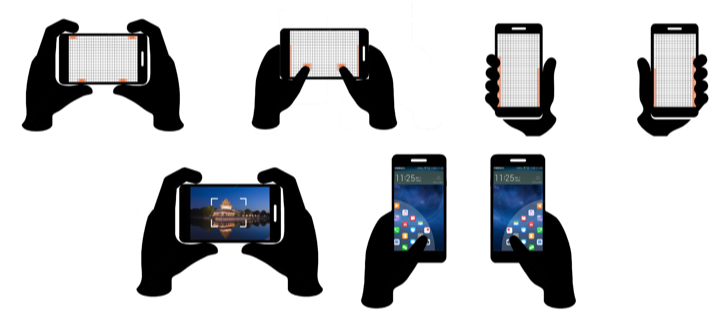
\includegraphics[width=0.95\columnwidth]{figures/hand-gesture.png}
    \setlength{\belowcaptionskip}{-6pt}
    \caption{Gesture sensing on edge of smartphone.}
    \label{fig:hand-gesture}
  \end{figure}

\subsection{Touch Interaction on the Back of Smartphone}
\textit{FlexTouch} can also extend the capacitive sensing capabilities to the back of the phone. This allows user to interact with a phone while it is placed in the pocket. In Figure ~\ref{fig:small-scale-scenarios}.D, we demonstrate an application where users can silence their phone during meetings leveraging capacitive touch enabled by \textit{FlexTouch} on the back of the phone. Please refer to the evaluation section for detailed implemention and study results. 

\begin{figure}[ht]
  \centering
    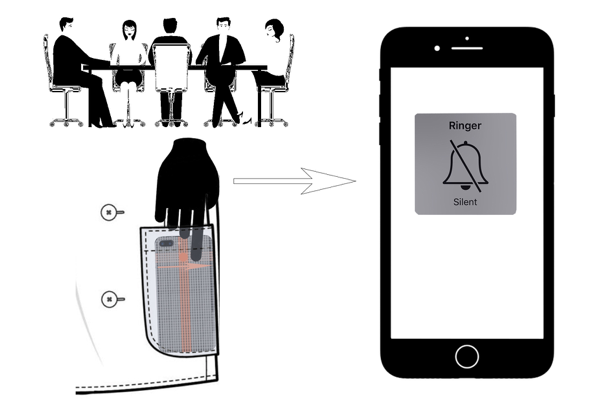
\includegraphics[width=0.95\columnwidth]{figures/backtouch.png}
    \setlength{\belowcaptionskip}{-6pt}
    \caption{Touch interaction on back of smartphone.}
    \label{fig:backtouch}
  \end{figure}

\subsection{Full-size Foldable Keyboard}
In Figure ~\ref{fig:small-scale-scenarios}.A, we designed a 29-key keyboard layout including character 'A'-'Z', \textit{Space, Enter, \emph{and} Backspace}. We fabricated three keyboards with different printed materials (carbon ink, ITO, silver ink) based on the designed layout. We utilized 29 pixels out of 32 along the edge of Huawei P20, and every key is linked to one sensing node on the screen. This allow us to enable full scale keyboard which can be easily attached onto the phone.

\begin{figure}[ht]
  \centering
    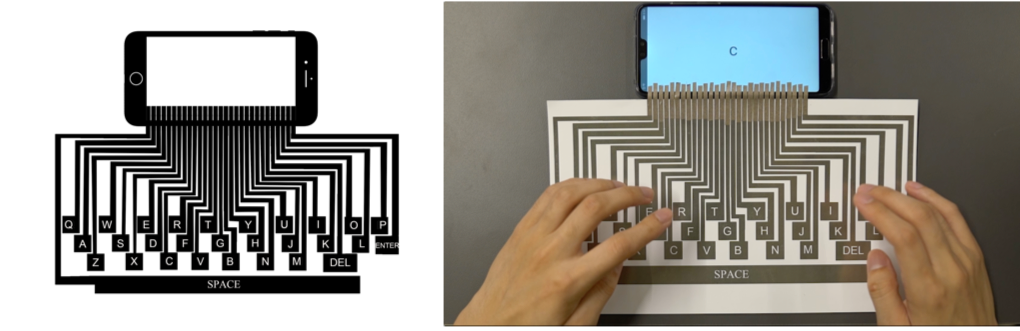
\includegraphics[width=0.95\columnwidth]{figures/keyboard.png}
    \setlength{\belowcaptionskip}{-6pt}
    \caption{Full-size keyboard using silver nanopartical ink-jet printing.}
    \label{fig:keyboard}
  \end{figure}

\subsection{Head-mounted {VR} Trackpad}
Phone based VR platform like the Google cardboard project mounts phones onto cheap and disposable cardboards for VR/AR applications. Such approach greatly lowered the barrier for VR hardware and allows easy access for developers to test out their VR/AR ideas. However, given the design of the cardboard approach, the touch screen is completely covered by the case and there is no easy way for  user to interact with digital contents. Figure ~\ref{fig:small-scale-scenarios}.B demonstrates an example where \textit{FlexTouch} wires out touch screen of phone to allow for touch interaction for phone based VR by allowing touch interaction on the cardboard surfaces on the back of the phone.

\begin{figure}[ht]
  \centering
    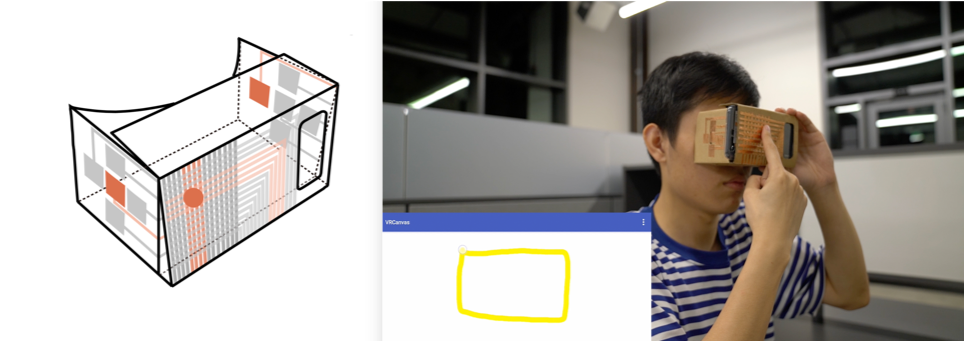
\includegraphics[width=0.95\columnwidth]{figures/vr-trackpad.png}
    \setlength{\belowcaptionskip}{-6pt}
    \caption{Enhanced VR interaction of back of smartphone.}
    \label{fig:vr-trackpad}
  \end{figure}


\section{Large-scale Interactions}

\subsection{Smart Mattress for Sleep Monitoring}
As \textit{FlexTouch}'s sensing range can reach up to 4 meters, we can leverage this long-range capability to detect users' behaviors while they're in bed. This is achieved by fabricating a three-layer structure with $5 \times 6 = 30$ sensing notes as presented in Fig ~\ref{fig:smartmattress} A - C. Each sensing node on the top layer is formed with a signal and a grounding electrode (Fig ~\ref{fig:smartmattress} B). All electrode pairs are connected to electrodes on the bottom layer. We placed a mattress on a wooden board and affixed a copper-tape circuit (Fig ~\ref{fig:smartmattress} C) with its electrodes connected with the electrodes on the bottom layer of the mattress. We activated the application by plugging in the touchscreen phone using a clip with an array of copper foil tapes attached (Fig ~\ref{fig:smartmattress} E to I). The material cost of this application was 10 USD.

\begin{figure}[ht]
  \centering
    \includegraphics[width=0.95\columnwidth]{figures/FlexTouch-mattress.png}
    \setlength{\belowcaptionskip}{-6pt}
    \caption{The structure of the smart mattress (A - C), the classification confusion matrix (D)  and the five detected states (E - I) with corresponding scenarios and raw sensing data visualization}
    \label{fig:smartmattress}
  \end{figure}

\subsubsection{User Evaluation}
To evaluate the performance of the smart mattress, we recruited eight pairs of participants (10 males) with an average age of 25.6 (SD = 2.2) and an average height of 170 cm (SD = 5.3) who we compensated with a \$20 gift card for a 30-minute test. There was one practice session followed by three data collection sessions. For each session, the paired participants followed the instruction of \textit{single user sitting on the bed}, \textit{single user lying on the bed}, \textit{one user sitting and one user lying on the bed}, \textit{two users lying on the bed} in order. The paired participants repeated the above procedure in each session five times and kept each posture for approximately 4 seconds. We logged the raw capacitive data with a Huawei P20 phone and logged the procedure with a camera for labeling. 

\subsubsection{Result}
All samples were manually labeled according to the video. We picked frames out of the series of data for each state. The dataset contains 120 data samples per posture across participants and each data sample includes 30 raw capacitive data points. The dataset was randomly split into 2 subsets (96 training samples and 24 testing samples). We conducted 5-fold cross-validation using the LibSVM classifier and achieved an average accuracy of 91.2\% across 5 states. We believe that the low resolution causes low recognition when users are sitting on the mattress, as Fig ~\ref{fig:smartmattress} D indicates. We discuss this result and future design recommendations in the later discussion section.   

\subsection{Smart Yoga Mat for Fitness Posture Detection}
The sensing range of \textit{FlexTouch} allows us to enable large-scale sensing applications such as a yoga mat.  \textit{FlexTouch} can detect and classify different user poses based on their capacitive profiles when working out on the yoga mat. Leveraging this functionality, smart home applications can adjust the surrounding environment based on users' physical activities. For instance, it could adjust ambient light, temperature, and music according to the user's activity on the yoga mat. The materials we used to build the touch-sensitive yoga mat cost just 8 USD. 

\begin{figure}[ht]
\centering
  \includegraphics[width=0.95\columnwidth]{figures/FlexTouch-yoga-new.png}
  \caption{Recognizing user's posture on the yoga mat built by \textit{FlexTouch} with raw sensing image data}  \label{fig:yogamat}
\end{figure}

As shown in figure ~\ref{fig:yogamat}, we built a 2D-patterned matrix ($8\times11 = 88$ sensing nodes) on a regular yoga mat using ITO strips, which can classify five different yoga poses (lord of the dance pose, plank, high lunge variation, camel pose and lotus pose).

\subsubsection{User Evaluation}
User Evaluation. We recruited 12 participants (6 males, 6 females, average age 27.7 (SD = 3.4), average height 171.2 cm (SD = 9.8). Each participant received \$10 for participating in this study, which included 1 practice session followed by three data collection sessions. Before each data collection session, the five postures were randomized. Then the participant performed each posture five times with a duration of 3 seconds. We logged the raw capacitive data with a Huawei P20 phone and logged the procedure with a camera for ground truth labeling.

\subsubsection{Results}
All samples were manually labeled according to the video. We picked the middle frame out of the series of data when the pose was performed. The dataset contains 180 data samples in total and each data sample includes 32 frames of raw capacitive data. We performed 5-fold cross-validation on the dataset (144 training samples and 36 testing samples for each iteration) using the LightGBM classifier and achieved an average accuracy of 97.1\% across 6 classes (five body postures and no action).

\subsection{Fitness Tracking on Count of Repetition, Speed and Distance}
In this example, we demonstrate fitness tracking applications when deploying \textit{FlexTouch} on a treadmill, cycling machine, and chest-press machine as shown in Figure ~\ref{fig:fitness}. Even though some recent commercial fitness machines have the function of sharing data to personal mobile devices, many machines are not embedded with this function such as chest press machine, lat pull-down gym machine, etc. Since these machines have similar periodic patterns, we propose these applications to inspire future designs by identifying the position where the sensing node is placed to sense states, state-changing events, and state-changing speed. We designed a binary sensor using a pair of $1.5m$-long, $3 mm$-wide copper foil tapes. Since the update rate of the Huawei P20 phone is 100 fps, the button sensor can detect not only the binary touch event but also how fast it changes. By counting the touch event frequency, we can calculate the distance or speed. This allows users to track their fitness behavior across devices at home or in the gym by simply plugging their phones into a customized passive module. Based on the tracking data, the application can customize fitness plans for individuals. This design cost 0.3 USD.

\begin{figure}[ht]
\centering
  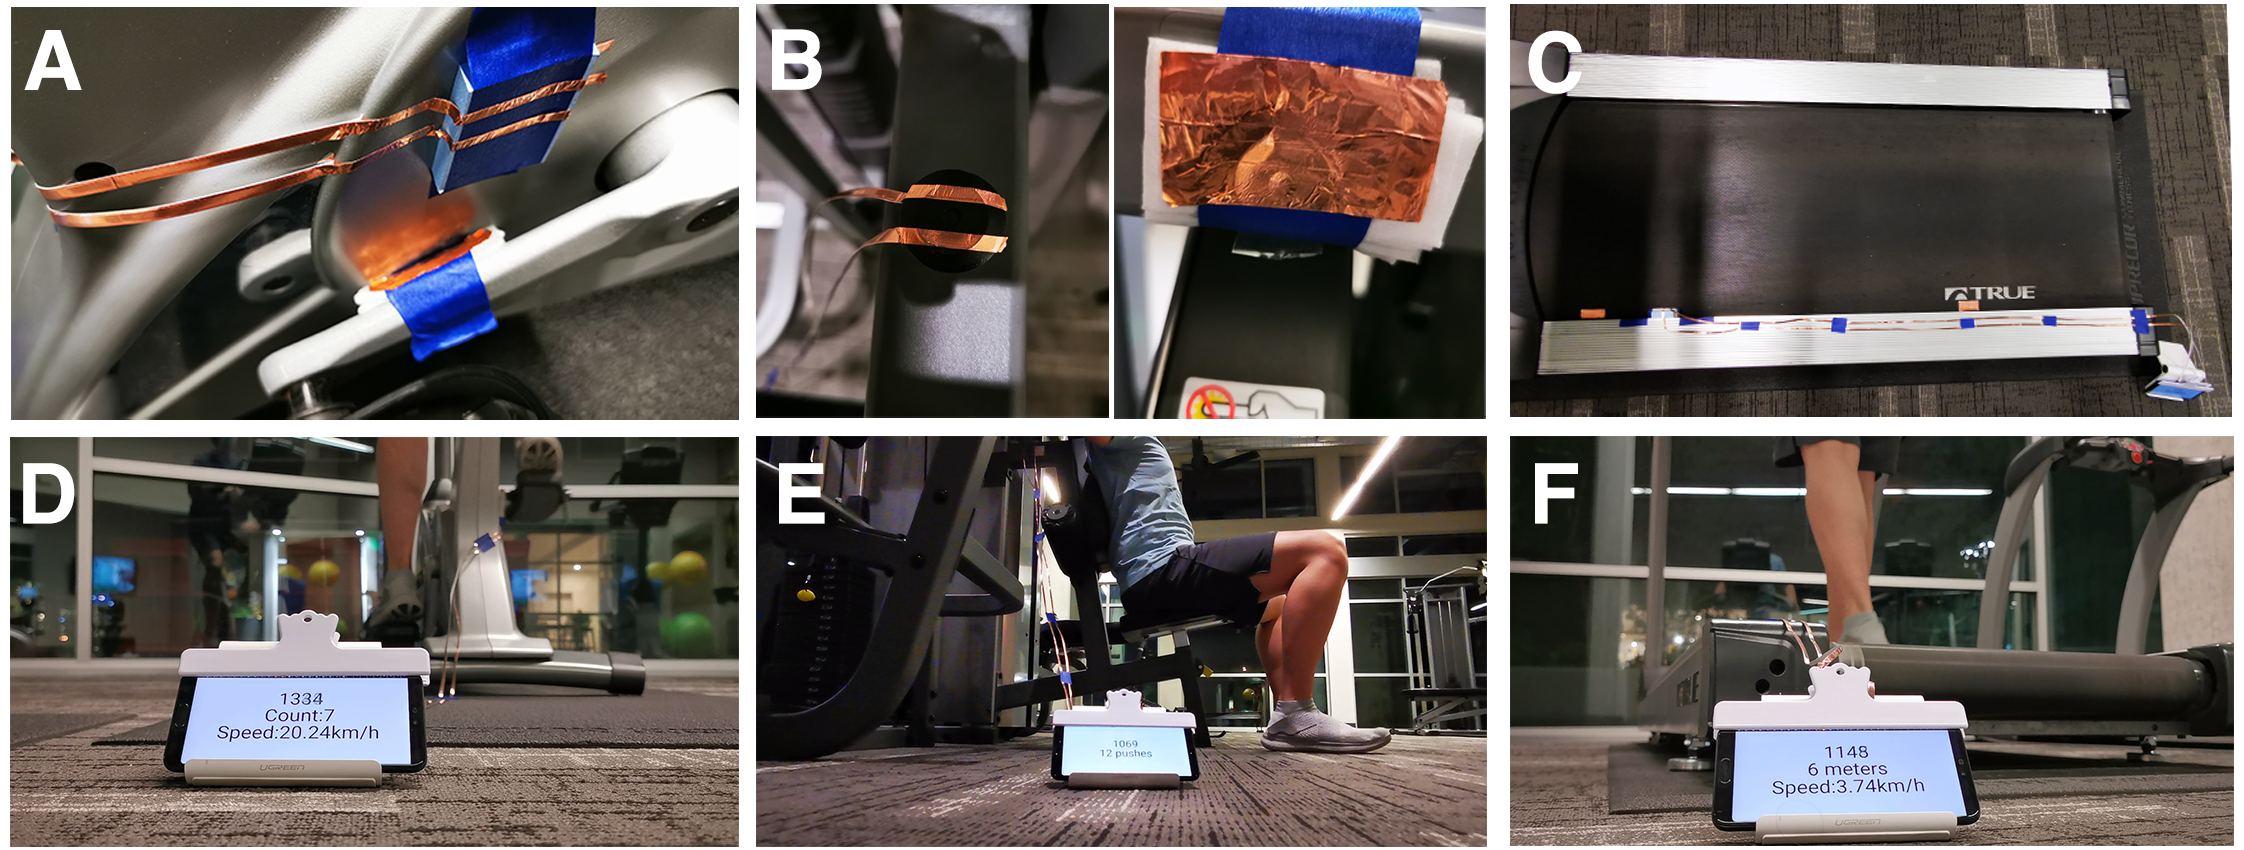
\includegraphics[width=0.95\columnwidth]{figures/gym.png}
  \setlength{\belowcaptionskip}{-4pt}
  \caption{Fitness tracking using \textit{FlexTouch}. A and D: speed tracking on a cycling machine. B and E: push counter on a chest-press machine. C and F: distance and speed tracking on a treadmill.}  
  \label{fig:fitness}
\end{figure}

\subsubsection{User Study}
To evaluate the tracking accuracy, we recruited six users (3 females, average age of 24.7 (SD = 0.8)). Each user finished three rounds of testing. For each round, users ran on the treadmill for 2 minutes with a maximum speed of $12KM/H$, rode the cycling machine for 2 minutes with a maximum speed of $25KM/H$, and, finally, finished the round with ten chest presses. The study lasted for 20 minutes and we compensated each participant with a \$20 dollar gift card. We used a camera attached on the display panel to record the speed and distance data from the fitness machine for ground truth annotation.

\subsubsection{Results}
We measured the maximum riding speed from the cycling machine, the maximum running speed and distance resolution from the treadmill as well as repeat counts from the chest-press machine. Since the signal processing algorithm stated in Section $4.4$ requires a minimum of 10 valid data to detect a touch event, there's an upper limit of the build button sensor's working frequency under 10 fps. Results indicate that \textit{FlexTouch} had an accuracy of 98.9\% on tracking the running and cycling speed and 100\% on tracking the chest-press count. Since the touch event happens once every cycle, our distance tracking resolution for the treadmill is 1.5 meter for the model that we tested.

\subsection{Smart Desk Reminder Application}
Given the flexible and passive nature of \textit{FlexTouch}, we recognize the potential to integrate it into large surfaces such as tables or desks to detect interaction with humans or everyday objects (Fig ~\ref{fig:smartdesk}). In this example, we placed three sensing nodes $40 cm$ away from the touchscreen to sense the user's body contact as well as one sensing node with $20 cm$ distance to sense the cup's water status (i.e. the amount of water remaining in the cup). When the user is working, instead of placing the phone on the desk, the user uses \textit{FlexTouch} to activate the smart desk application. It can remind users to take a break or stay hydrated by drinking water while they work continuously for a while. This is achieved by extending the touch sensing node to the desk where users lay their arm and place the water cup. The material cost for building this application was 0.30 USD.


\begin{figure}[ht]
\centering
  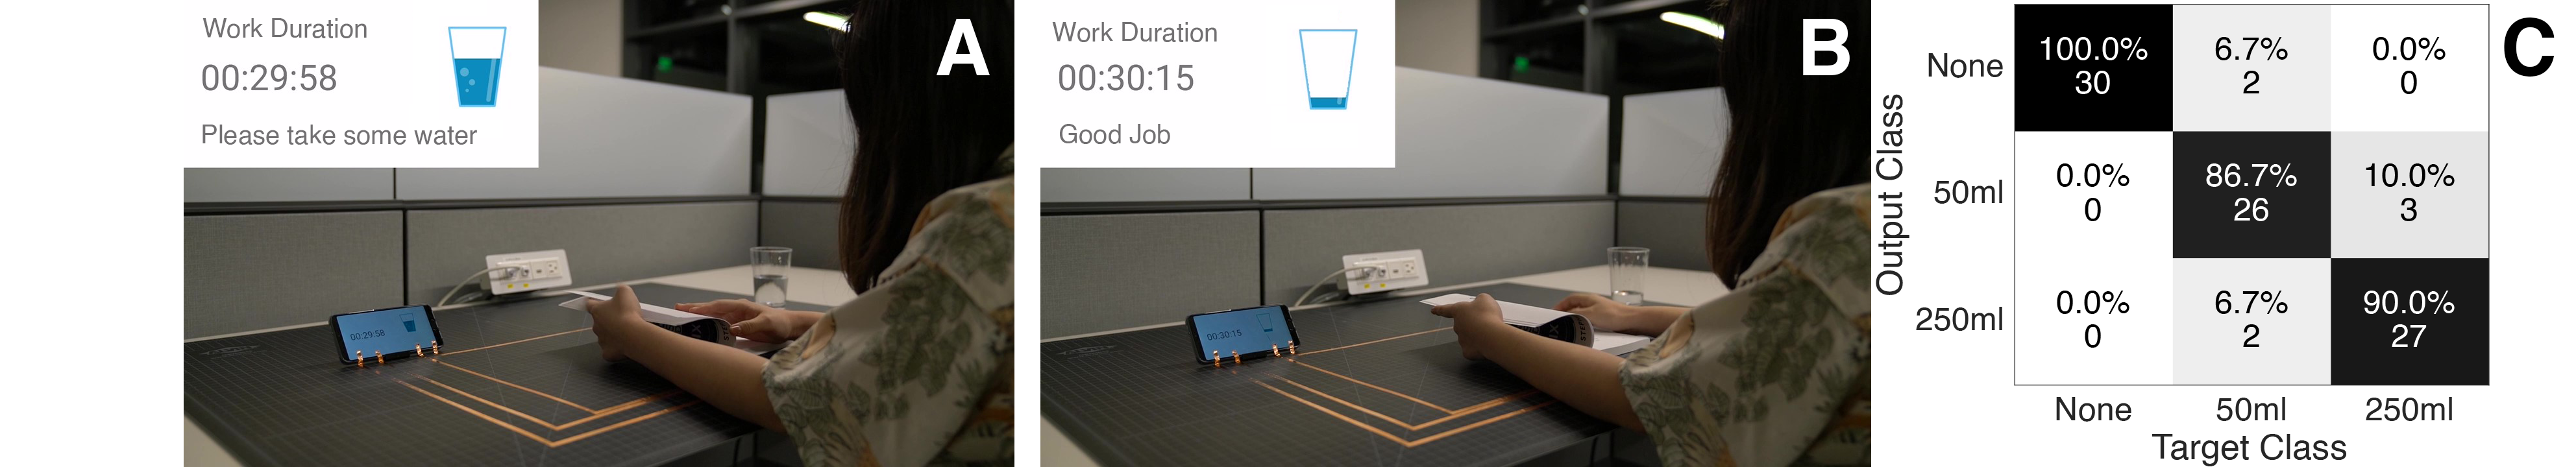
\includegraphics[width=0.95\columnwidth]{figures/FlexTouch-desk.png}
  \setlength{\belowcaptionskip}{-4pt}
  \caption{Smart desk example detecting user and object's presence and status}
  \label{fig:smartdesk}
\end{figure}

\subsubsection{User Study}
To evaluate the sensing performance on the presence and status of the user and the water cup, we conducted a user study in which six users (2 females, 4 males, average age of 25.0 (SD = 0.9)) participated. For each round, users read a book with his or her arms laying on the table for 20 seconds and then replaced the thin plastic water cup filled with $250 ml$ water with another water cup filled with $50 ml$ water. Finally, the user left the desk for 10 seconds and came back to repeat the session five times in total.

\subsubsection{Results}
We obtained a dataset containing 16 minutes of user's behavior data ($96.5 K$ data frames). We manually labeled the data to extract 60 data points on user presence status and 90 data points on the cup status. We measured the detection accuracy by whether the user was present as well as the cup's water status (not present, $50 ml$ and $250 ml$ water inside). Results show that \textit{FlexTouch} can achieve an accuracy of 98.3\% on in detecting the user presence at the desk, an accuracy of 92.2\% on the cup water status (see the confusion matrix in Figure \ref{fig:smartdesk} C).

\section{Summary}
In this chapter, we proposed a set of different applications that \textit{FlexTouch} can be easily applied. First, we showed four example applications of smartphone ambient interaction under common user scenarios. Different from prior work, based on the signal processing technique we described in chapter 4, we are able to provide a broader range of ambient interactions without any disturbance of user's usual on-screen interactions. Then we presented several large-scale interaction examples along with concrete user study and result analysis. The results demonstrated the feasibility and roubustness of \textit{FlexTouch} in large-scale settings.